\documentclass[11pt]{article}

\usepackage{a4wide}
\usepackage{mathptm}
\usepackage{xspace}
\usepackage{amsmath}
\usepackage{graphicx}
\usepackage{algorithm}
\usepackage{algpseudocode}
\usepackage{tikz}
\usepackage{tkz-graph}
\usetikzlibrary{shapes.misc, positioning}
\usepackage{listings}
\usepackage{color}

\definecolor{dkgreen}{rgb}{0,0.6,0}
\definecolor{gray}{rgb}{0.5,0.5,0.5}
\definecolor{mauve}{rgb}{0.58,0,0.82}

\lstset{frame=tb,
  language=Java,
  aboveskip=3mm,
  belowskip=3mm,
  showstringspaces=false,
  columns=flexible,
  basicstyle={\small\ttfamily},
  numbers=left,
  numberstyle=\tiny\color{gray},
  keywordstyle=\color{blue},
  commentstyle=\color{dkgreen},
  stringstyle=\color{mauve},
  breaklines=true,
  breakatwhitespace=true,
  tabsize=3
}
\begin{document}

\title{DAT 250\\Advanced Software Technologies}

\author{Wojciech Pasiak\\Christoffer Brandhaug\\Erlend Meling Torsvik\\Jaroslaw Pasiak}

\maketitle

\rule{\textwidth}{1.6pt}\vspace*{\baselineskip}\vspace{2pt}
\vspace{0.75\baselineskip}
{\huge \centering
Feed App Project\\}
\vspace{0.75\baselineskip}
\rule{\textwidth}{1.6pt}\vspace*{-\baselineskip}\vspace{2pt}
\vspace{9pc}
\begin{figure}[H]
  \centering
  
\includegraphics[scale=0.5]{figs/HVL_logo.jpg}
  \label{fig:logo}
\end{figure}
\newpage
\tableofcontents
\newpage

\begin{abstract}

  10-15 lines with the software technology and the highlights from the
  project that has been undertaken.

\end{abstract}

%\input{commands}

\section{Introduction}
\label{sec:introduction}

Approximately 1 page on:

\subsection{Implementation}
\label{sub:implementation} A brief introduction to the prototype implementation and topic of the project.

\subsection{Technology stack}
\label{sub:techstack} Discuss (briefly) the technology stack that has been selected, mention related technologies (if relevant), primary arguments for choice of technology stack.

\subsection{Results}
\label{sub:results} A brief account of the results that have been obtained in the project.

\subsection{Organization of report}
\label{sub:organization}A one paragraph overview at the end, explaining how the rest of the report is / has been organised.

\noindent
This rest of this report is organised as follows:
Section~\ref{sec:technology} gives an ....


\section{Software Technology Stack}
\label{sec:technology}

This section of the report will cover each of the chosen software technologies that are implemented in the final project application. It will introduce some of key concepts of the technologies, with some running examples. 

\subsection{Firebase}
\label{sub:firebase}
Firebase is a Backend-as-Service (BaaS) platform created by Google that provides helpful tools. Examples of these are:

\begin{itemize}
 \item \textbf{Firebase Database:} Is a NoSQL cloud database used for storing and syncing data. The data is synced in realtime and remains available even when the application goes offline. The data is stored as JSON. \cite{firebasedb}
 \item \textbf{Firebase Cloud Firestore:} Cloud database with good scalability for mobile, web and server development. Cloud Firestore offers flexibility, expressive querying, realtime updates and more. \cite{firebasefs}
 \item \textbf{Firebase Cloud Messaging:} Used to send notification/data messages. \cite{firebasecm}
 \item \textbf{Firebase Remote Config:} Used to quickly update/change behavior and appearance of your application without having to download an update. \cite{firebaserc}
\end{itemize}
As for the poll application that was made in the project it only uses the Cloud Firestore out of these four. In the Cloud database the data is stored in documents with underlying collections where all values are stored in a structural way. In Figure~\ref{fig:fb} the data is stored in such a way, with IDs as the document name and the values are stored in collections with fields for each value. The database supports many different data types, from integers and strings to more complex data in the form of objects.
\begin{figure}[H]
  \centering
  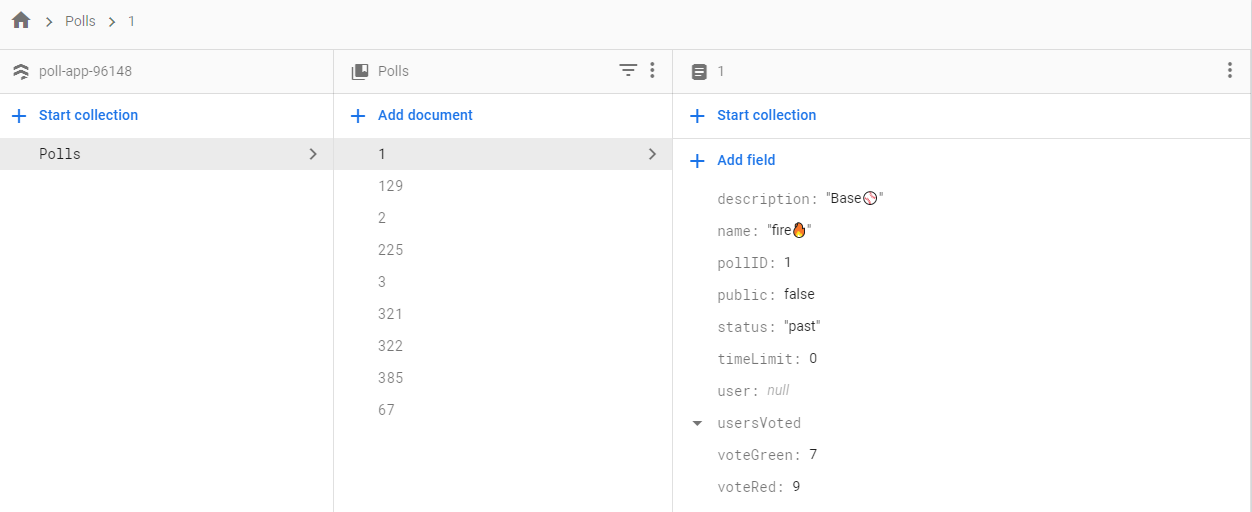
\includegraphics[scale=0.4]{figs/fb.png}
  \caption[scale=0.5]{Firebase Cloud Firestore.}
  \label{fig:fb}
\end{figure}

\subsection{RabbitMQ}
\label{sub:rabbitmq}

RabbitMQ is an open source message broker that implements Advanced Message Queuing Protocol (AMQP). RabbitMQ is an intermediary for messaging. “It gives your applications a common platform to send and receive messages, and your messages a safe place to live until received.” \cite{rabbitftrs}
How this works is that a producer publishes messages to the “exchange” with specific type of exchange, the exchange then delivers the messages to different queues depending on exchange types. The recipients will then retrieve messages which they have subscribed to.

\subsection{Spring framework}
\label{sub:spring}
\subsubsection{Thymeleaf}
Thymeleaf is a template engine written in Java for HTML5/XHTML/XML. It can be used in both web and non-web environments. Thymeleaf implements the concept of Natural Templates, that are described as: “template files that can be directly opened in browsers and that still display correctly as web pages” \cite{thymlf}. The use of Thymeleaf can act as a replacement for using Java Server Pages \cite{javaserverpages}.
\subsubsection{Spring Boot}
Spring Boot allows for creating Spring based applications in an “easy” way that just runs, with minimal effort. Spring Boot does a lot of the configuration for the user by being a framework built on top of Spring framework which enables the user to quickly “bootstrap” a Spring application from scratch. The Spring initializer makes for an effortless start to any project by simply picking out dependencies according to the type of project.
\subsubsection{Spring JPA}
Spring JPA is a framework provided by Spring, to make it easier for developers to implement data access layer. By letting the developer only have to write the entities, repository interfaces, and perhaps making some extra custom repository searching methods. While the developer is focusing on programming the vision of the project, Spring JPA will implement all necessary methods for accessing all the data from repositories for the developer.
\subsubsection{Spring MVC}
Spring MVC is the framework used to build the web application. It provides the Model-View-Controller architecture. This simply means that it separates the application into a model, view, and controller component. The task of these components is to handle different sides of the development in an application. When it comes to creating scalable projects, Model-View-Controller is one of the most commonly used web development frameworks.
\subsubsection{Spring Security}
Spring Security is a powerful and highly customizable authentication and access-control framework. It is the the most used and a practical standard for securing Spring-based applications, thus also our application. Spring Security is a framework that focuses on providing both authentication and authorization to Java applications.\cite{springsecurity} Security is very important and should not be taken for granted. In this aspect, Sprint Security makes it very easy to customize and tweak the settings to meet the developers preferences. Features available to customize is a long list, but protection against attacks and authentication with access-control (AC), are the few features that are featured in our FeedApp application.
\subsection{Dweet.io}
\label{sub:dweet}
Dweet.io is a type of messaging system for machines. It is also referred to as a “Twitter for social machines” \cite{dweet}. A machine can either publish or subscribe to data, and all data published to dweet.io can be retrieved by simply calling an URL. All messages published to dweet.io will be associated with an unique name. The data is structured in JSON format. 

\subsection{H2 Database}
\label{sub:h2db}
H2 Database is an open-source SQL database written in Java. The database can be embedded in Java applications, making it a suitable choice for development and testing. The database engine is also exceptionally fast. \cite{h2db} 

The H2 console allows for a full view of the database. It allows for SQL commands for inspecting/or changing values in the database, as is seen in Figure~\ref{fig:h2console}. After starting an application with H2 embedded in it, the console can be reached in a browser by calling the path URL that is configured. If the application is running on port 8080, and the path URL is set to /h2-console, simply call “localhost:8080/h2-console”. After inputting the correct username and password, one is free to inspect and manage values the database. 
\begin{figure}[H]
  \centering
  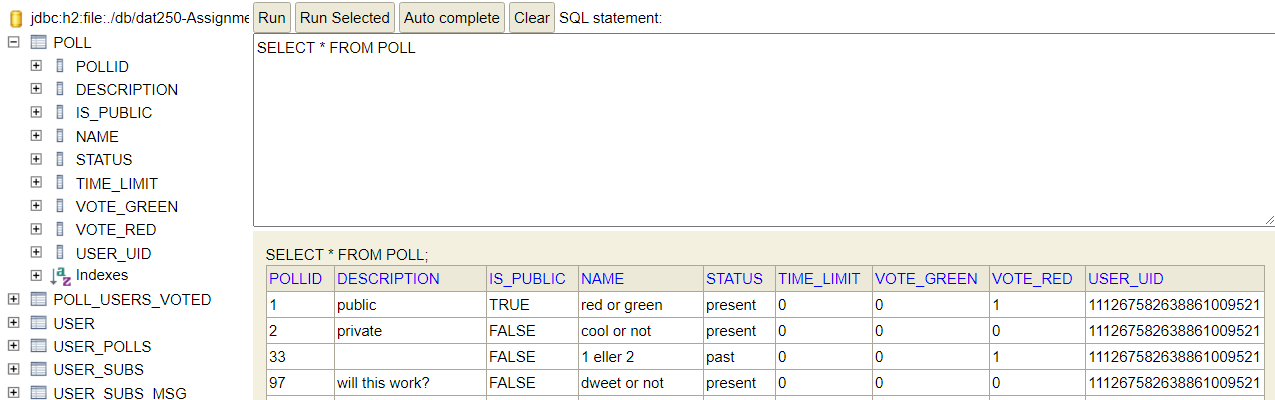
\includegraphics[scale=0.45]{figs/h2cons.png}
  \caption[scale=0.5]{A SQL command is run in the H2 console.}
  \label{fig:h2console}
\end{figure}

\section{Demonstrator Prototype}
\label{sec:design}

In this project, several software technologies were used that have already been mentioned and described in section above. For all technologies to communicate with each other, a REST API is used. User can view the application by sending HTTP request to server from web browser and server replying with a handled response. A user has different "interaction" he/she can do with the web application, those are described in Section~\ref{sub:usecase}.

\subsection{Architecture}
\label{sub:architeure}
Figure~\ref{fig:archdiagram} represents the architecture diagram for the FeedApp.
A Client (user) uses the web browser to send requests and get responses from the server (application). To use the application the user needs to be authenticated (logged in), at least for the most use cases of the application. Requests gets handled by the REST API on the server which processes the request and sends a response accordingly. REST API communicates with the database to save/get persisted data.

There is also support for IoT devices to communicate with the server, and it sends the requests straight to the REST API which doesn't have to go through the extra steps with authentication and Model view in web browser.

This project additionally includes a messaging system that gets poll information from REST API and sends them to a NoSQL database. Where the polls can be used in other use cases, than the web application intends to.
\begin{figure}[H]
  \centering
  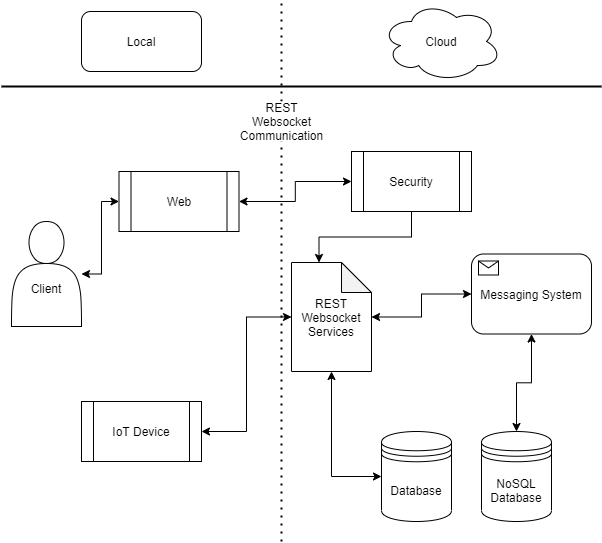
\includegraphics[scale=0.5]{figs/archdiagram.png}
  \caption[scale=0.5]{Architecture diagram.}
  \label{fig:archdiagram}
\end{figure}

\subsection{Application flow}
\label{sub:appflow}
Application flow can be seen in Figure~\ref{fig:applicationflow}, which has the thought out interactions on the different web pages and what will be possible for the user to do. A users will be able to vote on a public poll without the need of being authenticated, or be in possession of an account at all. If the poll is private, then the user will be able to create an account to vote. After creating an account, user will have the opportunity to create/edit his/her own polls. User needs a PollID to vote, and to find the different PollIDs, an option to search for available polls by their respective names will be created. 

Some actions can end in a failure, these will be handled with proper responses giving the user "detailed" information on what to correct, for the different actions.
\begin{figure}[H]
  \centering
  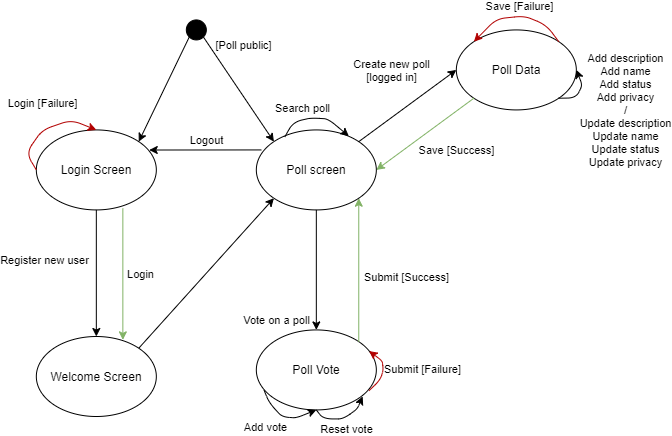
\includegraphics[scale=0.5]{figs/applicationflow.png}
  \caption[scale=0.5]{Application flow.}
  \label{fig:applicationflow}
\end{figure}

\subsection{Use case}
\label{sub:usecase}
In Figure~\ref{fig:usecases}, user enters the Application via web browser and is able to login or register new account. On main page after logging in; user can create a new poll, delete or edit an already existing poll (if user is owner), search/look-up a poll and vote on it. Since the application also supports IoT devices, the use case of an IoT device is to enter a poll with PollID and vote on it.

\begin{itemize}
  \item \textbf{Vote on a Poll:} Everyone can vote on a public poll, using a web form, but to vote on a private poll the user must be logged in.
  \item \textbf{Register:} Everyone can register a new account to use the web application services, using OAuth.
  \item \textbf{Create Poll:} A logged in user can create a new poll using a web form.
  \item \textbf{Subscribe to Poll:} A logged in user can subscribe to a poll after entering the voting screen with PollID.
  \item \textbf{Show own polls:} A logged in user can view his/her own created polls, including the "live" voting results.
  \item \textbf{Show subscription messages:} A logged in user can view messages from subscriptions, on subscribed polls.
  \item \textbf{Delete Poll:} A logged in user can delete own polls from show own polls screen.
  \item \textbf{Edit Poll:} A logged in user can edit his/her own polls, using another web form from show own polls screen.
  \item \textbf{Look-up a Poll:} Everyone can look-up a public poll by the name, but only logged in users can look-up private polls.
  \item \textbf{IoT Device:} An IoT device can vote on all polls with known PollID. IoT can also see Poll data, with-it the results as well.
\end{itemize}
\begin{figure}[H]
  \centering
  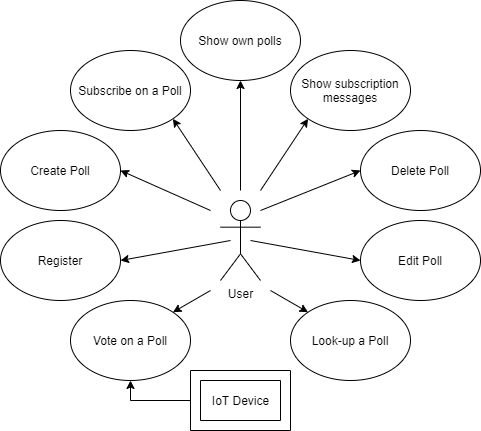
\includegraphics[scale=0.5]{figs/usecases.png}
  \caption[scale=0.5]{Use cases.}
  \label{fig:usecases}
\end{figure}

\subsection{Domain model}
\label{sub:domainmodel}
The domain model in Figure~\ref{fig:domainmodel} describes the planned persisted entities. A User with a uID as primary key can have multiple Polls, with a PollID as primary key and User as a foreign key. The database will also save which user has voted on which poll, so that a logged in user cannot vote multiple times on the same poll. This data is persisted into "User has Voted" table.
\begin{figure}[H]
  \centering
  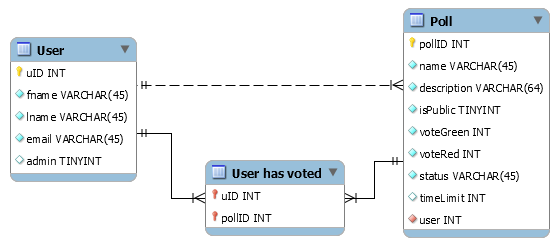
\includegraphics[scale=0.5]{figs/domainmodel.png}
  \caption[scale=0.5]{Domain model.}
  \label{fig:domainmodel}
\end{figure}

The user also has lists of Polls he/she subscribed to, to receive updates, and subscription message list, with messages from the subscriptions.

\par\noindent In the next section implementation of the project will be covered, and the different technologies used.

% This section should provide details of how the prototype has been implemented which may involve presentation of suitable code snippets.
\section{Prototype Implementation}
\label{sec:implementation}
In this section we'll describe how the different software technologies were implemented and how they were used in our project, by briefly mentioning what they do and how we thought by implementing them. Code snippets are also showed to explain and visualize how the code looks in our real-time project.

\subsection{JPA}\label{sub:jpa}
Prototype implementation had few major steps. First and most crucial one, was to create JPA entities and let them communicate with each other, from given relations between them.

Two entities were created, \textbf{POLL} and \textbf{USER} with appropriate relations stored in Derby H2 relational database. Relations between those entities are One-To-Many, since one user can create many polls, but only one user can be the creator/owner of a specific poll. Furthermore, there is a possibility to vote on a specific poll, thus there is a need for storing data about that too. This is handled with a "Many-To-Many" relation between Poll and User entities, creating a new table with two attributes \textbf{User.uID} and \textbf{Poll.pollID} storing "who voted on what".

As shown in the example below, JPA makes it very easy to create new entities. Just by adding annotation \textit{@Entity}, the Java class is then declared to behave as an entity when program runs. In the same way we can use \textit{@Id, @ManyToOne, @ManyToMany, ...} annotations to configure the desired relations and identities for different entity attributes.

\lstinputlisting[language=java]{code/pollentity.java}

JPA doesn't give basic; create, read, update and delete (CRUD) operations, when new entities are created. Therefore, it was necessary to create own Data Access Object (DAO), for every entity created. This is very cumbersome and time consuming. Benefits of using Spring Framework, is that CRUD operation can very simply be added for entities by extending a Spring Framework Class (CrudRepository or PagingAndSortingRepository which extends CrudRepository), we chose PagingAndSortingRepository, as it has the same functionalities as the other class, but with some extra functions which make it simpler to "page and sort" the results obtained.  

In the code snippet below, we can see our implementation of User repository extending the spring framework class. With an extra functionality, \textit{findByFname}, which is a read operation to search for a user by his/her first name.

\lstinputlisting[language=java]{code/userrepo.java}

\subsection{REST}\label{sub:rest}
With the entities set up and ready to be used, a user needs some way to interact with this data. To accomplish this, a REST API needs to be implemented. To implement a business logic side, Spring Framework was used again. With the benefits of using Java annotations \textit{@Controller}, the Java class is then declared to behave as a RestController when program runs. Creating new methods within this Class and annotating them with desired mapping annotation, all CRUD operations can be accessed from HTTP requests.

\lstinputlisting[language=java]{code/pollrest.java}

As we can see in the code snippet above, it is very simple to use Spring frameworks annotation to also make a REST controller. The \textit{@Controller} annotation, makes this class a controller when the program runs. To use different repositories to use in this controller class, we need some way to access them, this is accomplished with the annotation \textit{@Autowired}, which wires the repository to the controller when the program launches.

In a controller class we can use different request mappings, such as \textit{@GetMapping} and \textit{@PostMapping}, which we used in our code. In the different request mappings, we need to define the path at which to access the different methods. In the code snippet there are two examples of such mappings, one POST mapping, which at the path \textit{/pollAdd}, needs parameters defined with \textit{@RequestParam} to execute the \textit{pollAdd()} method. And a second, GET mapping to search polls at the path \textit{/polls} with defined parameters.

While implementing REST API to our prototype; post, get, put, delete mapping was used to make user interact with prototype's business logic. Since this requires the user to send HTTP-request with different mappings for different operations. Later, this was modified and downgraded to only GET and POST mappings, since those are the only two HTTP requests a HTML form supports.

\subsection{Security}\label{sub:security}
Since a user must register and login to use most parts of the web page, there needed to be some security implemented. For this we used Spring frameworks Security dependency, which allowed us to simply define which pages could, and which couldn't be accessed without logging in, this can be seen in the code snippet below.

For a “simpler” and more secure login process, we decided to use Google's OAuth 2. By doing this, we don't need to store sensitive user information, and user doesn't need to create a new password for him/her to remember. As the best security is the security you don't need to implement yourself, which can cause unintended errors or follow with security holes.

\lstinputlisting[language=java]{code/security.java}

{\footnotesize\textbf{Disclaimer!}\textit{ All documentations and tutorials we looked at about Spring Framework were taken from \cite{spring_Framework}}}

\subsection{Firebase}\label{sub:firebase}
\textbf{\textit{TODO}}

\subsection{Messaging System}\label{sub:messaging}
In the web application, a user can subscribe to a poll and receive its results when the poll closes. This calls for a messaging system implantation. For this we used RabbitMQ with a receiver and a sender class, again using Java annotations to declare a method to be a RabbitListener. We chose to use a topic-based messaging queue, as it made it easy to use poll status (present, past, future) as the topic keys.

But before a user can receive messages from a subscription, the user must subscribe to a specific poll, which is then saved in a subscription list that the user has saved in its entity. From these lists, rabbit listener finds correct receivers and sends the requested message to them. 

\subsection{Front End}\label{sub:frontend}
User interacts with the program via web browser and gets information from database by communicating with business logic via Spring MVC, using Thymeleaf. Thymeleaf is an integrated method to use in HTML code in order to access data from models, generated based on the request sent by user. HTML code was used to create different use case screens and according to what requests can be made, the appropriate thymeleaf code was inserted into HTML code. For the pages to look "better" and be user friendly with what can be done on a web page, CSS was used to decorate the pages and how they look/show up for the client.


\section{Test-bed Environment and Experiments}
\label{sec:evaluation}

About 2 pages that:

\begin{description}
\item[Explains] how the prototype has been tested the test-bed environment.

\item[Explains] what experiments have been done and the results.

\end{description}

For some reports you may have to include a table with experimental
results are other kinds of tables that for instance compares
technologies. Table~\ref{tab:results} gives an example of how to create a table.

\begin{table}[H]
\centering
\begin{tabular}{llrrrrrr}
  Config & Property & States & Edges & Peak & E-Time & C-Time & T-Time
  \\ \hline \hline
22-2 & A   &    7,944  &   22,419  &  6.6  \%  &  7 ms & 42.9\% &  485.7\% \\
22-2 & A   &    7,944  &   22,419  &  6.6  \%  &  7 ms & 42.9\% &  471.4\% \\
30-2 & B   &   14,672  &   41,611  &  4.9  \%  & 14 ms & 42.9\% &  464.3\% \\
30-2 & C   &   14,672  &   41,611  &  4.9  \%  & 15 ms & 40.0\% &  420.0\% \\ \hline
10-3 & D   &   24,052  &   98,671  & 19.8  \%  & 35 ms & 31.4\% &  285.7\% \\
10-3 & E   &   24,052  &   98,671  & 19.8  \%  & 35 ms & 34.3\% &  308.6\% \\
\hline \hline
\end{tabular}
\caption{Selected experimental results on the communication protocol example.}
\label{tab:results}
\end{table}


\section{Conclusion}

This project has introduced some great learning experiences, together with a decent amount of challenges along the way. The first step was learning about all the different software technologies, both the ones introduced in the course, and the additional ones that were included in the application like Firebase and H2 database. The biggest challenge might have been understanding how relations between entities worked in a relational database, and how to configure them in a proper way. These entity classes also had to be integrated with the Spring application. This made the learning curve relatively steep for the earlier parts of the project. Luckily, the Spring framework documentation covers a vast variety of topics, and there are a multitude of guides on how to integrate different technologies with Spring.

This made the learning curve flatten a bit after getting a decent understanding of each of the technologies. However, even with associated guides, not every technology behaved as expected when trying to implement them. Originally, the project was supposed to use MongoDB \cite{mongodb} as the non-relational database. Implementing MongoDB with the H2 database turned out to give some unexpected errors, and after a few days of trial and only getting errors it was decided to use Firebase as the non-relational database instead. This was fortunately the only major speedbump that the project hit. Implementing the messaging system with RabbitMQ and Dweet.io was for the most part unproblematic, using the respective technologies own documentation for understanding their core concepts and how to utilize them properly. 

The reference list includes a set of online sites used throughout the project when learning about the different technologies and examples of how to implement them into other projects. Most of the references listed are for the software technologies not introduced in the course.



\bibliographystyle{plain}
\bibliography{report}

\end{document}
